% \documentclass{book}

\documentclass[12pt]{article}
\usepackage[pdfborder={0 0 0.5 [3 2]}]{hyperref}%
\usepackage[left=1in,right=1in,top=1in,bottom=1in]{geometry}%
\usepackage[shortalphabetic]{amsrefs}%
\usepackage{amsmath}
\usepackage{enumerate}
\usepackage{enumitem}
\usepackage{amssymb}                
\usepackage{amsmath}                
\usepackage{amsfonts}
\usepackage{amsthm}
\usepackage{bbm}
\usepackage[table,xcdraw]{xcolor}
\usepackage{tikz}
\usepackage{float}
\usepackage{booktabs}
\usepackage{svg}
\usepackage{mathtools}
\usepackage{cool}
\usepackage{url}
\usepackage{graphicx,epsfig}
\usepackage{makecell}
\usepackage{array}

\def\noi{\noindent}
\def\T{{\mathbb T}}
\def\R{{\mathbb R}}
\def\N{{\mathbb N}}
\def\C{{\mathbb C}}
\def\Z{{\mathbb Z}}
\def\P{{\mathbb P}}
\def\E{{\mathbb E}}
\def\Q{\mathbb{Q}}
\def\ind{{\mathbb I}}

\graphicspath{ {images15/} }

\begin{document}

\section*{10 May 2017}

\subsection*{Some Checks}

\subsubsection*{Energy growth/decay?}

Here we want to look at the change in energy around our (supposed) center, i.e. Double Pulse 2. If the eigenvalue is in fact pure imaginary, we should have periodic orbits. If there is a real part, we should have a spiral, with direction given by the sign of the real part. For $N =256$ grid points and c = $9.4812$, the initial eigenvalue we get from \texttt{eig} is $1.2910e-11 \pm 0.0629i$. For $N = 1024$ grid points, the real part is 1.5738e-08.\\

The question is whether this small real part is ``real'' or not. Two pieces of evidence suggesting that the real part should be zero are:
\begin{enumerate}
	\item We can use \texttt{fsolve} to eliminate the small real part and get a better value for $\max |Lf - \lambda f|$, suggesting that the small real part is numerical error.
	\item \texttt{eig} gives two other small eigenvalues at -2.8590e-06 and 2.8589e-06 whose eigenfunctions are the derivative of the double pulse. We know these two eigenvalues should both be 0, since there is a double eigenvalue at 0 whose eigenfunction is the derivative. This real part is larger than the real part for the complex eigenvalue. If we increase the number of grid points, these eigenvalues approach 0.
\end{enumerate}

The problem is that we cannot be sure there is not a very small real part to this eigenvalue. We can obtain a further piece of evidence by looking at how the solution $u(t)$ changes with time. If $\alpha$ is the real part of the eigenvalue, than the peak height should (roughly) change according to
\[
|u(t)| = e^{\alpha t} |u(0)|
\]

So we should see how many time steps we need to run until we see a change in $|u(t)|$, e.g. for it to double/half. Unfortunately, the number is so large that it is not feasible to actually do this. A rough calculation is as follows. For $N = 256$, $c = 9.4812$, the nonzero eigenvalues are $1.2910e-11 \pm 0.0629i$. The real part here is much smaller than we had found originally (about 1e-6) and results from us enforcing a symmetry condition on the double pulse. If we want the magnitude of the oscillations to double (not unreasonable, since that would be visually apparent), then we need to integrate to:

\[ t = \log(2) / 1.2910e-11 \approx 7e10 \] 

Since each time step is 0.01, we need approx 7e12 time steps, which is not feasible.

\subsubsection*{Time-stepping around stationary solutions}

Here we do our time-stepping procedure around our stationary solutions to see if we have any small oscillations. For Double Pulse 2 (our ``center''), we take 100000 time steps, size 0.01 each, sampling every 5 steps. Here is a plot of derivative of peak distance vs peak distance, before and after FFT smoothing

\begin{figure}[H]
	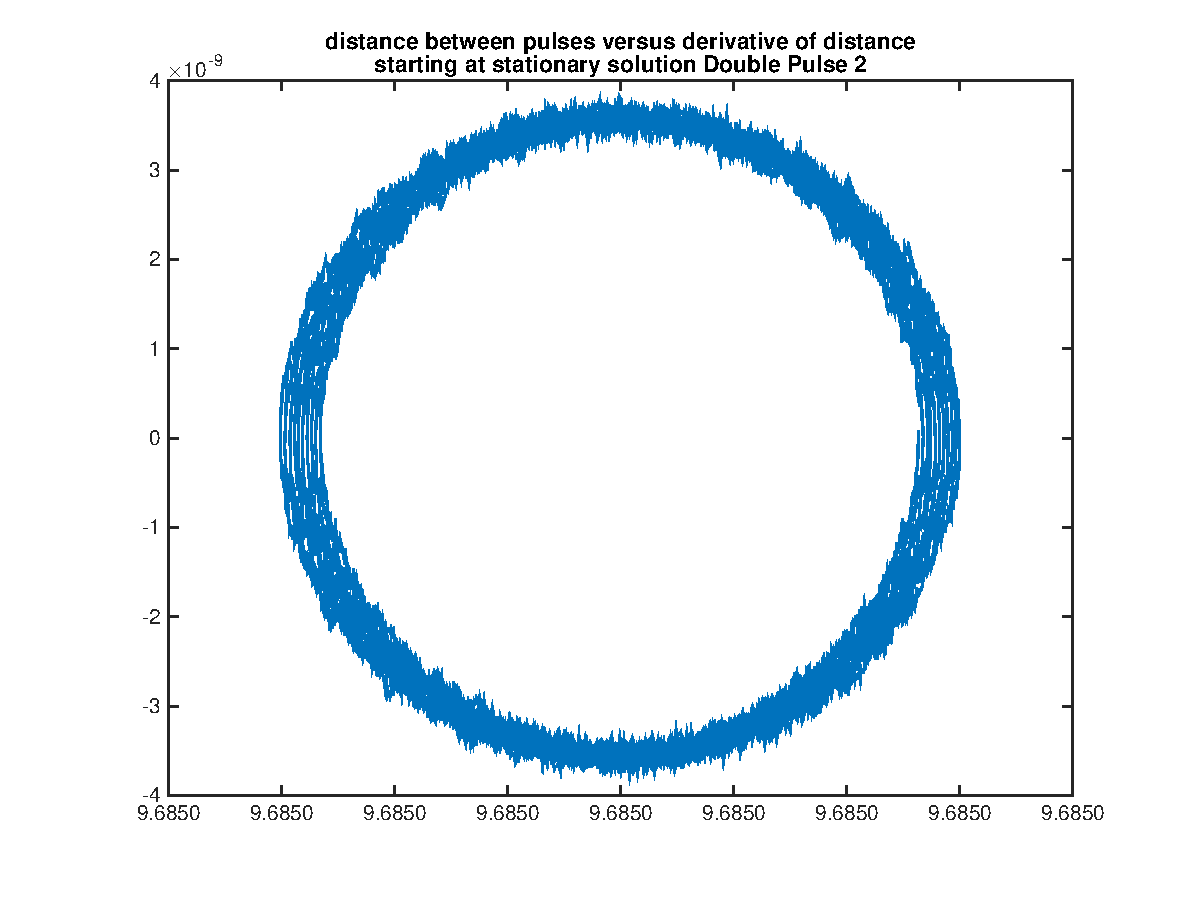
\includegraphics[width=8.5cm]{stationary1a.eps}
	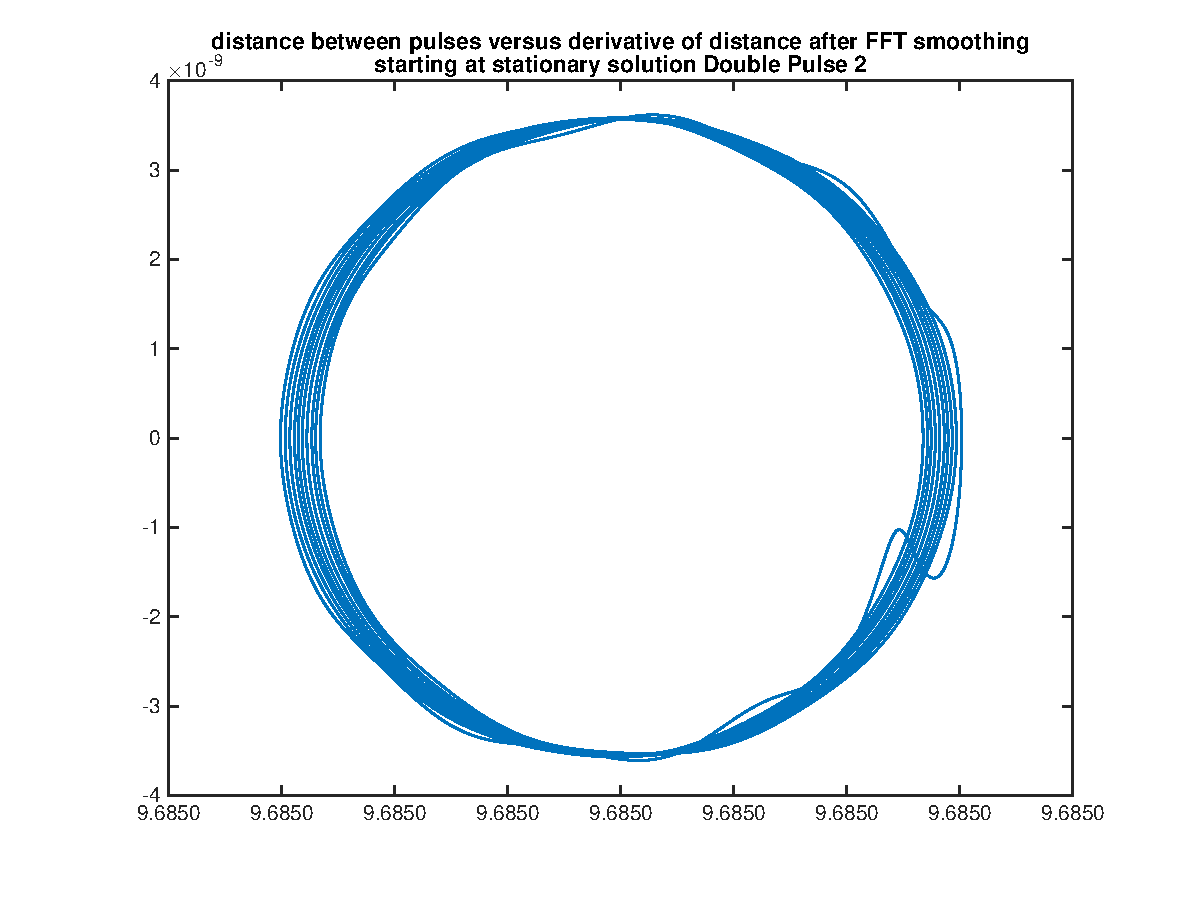
\includegraphics[width=8.5cm]{smoothstationary1a.eps}
\end{figure}
We see that there are small, high-frequency oscillations here. The peak distance is also increasing (on average) ever so slightly with time. We can look at plots of the L2 norm of the solution vs time and the peak distance vs time.

\begin{figure}[H]
	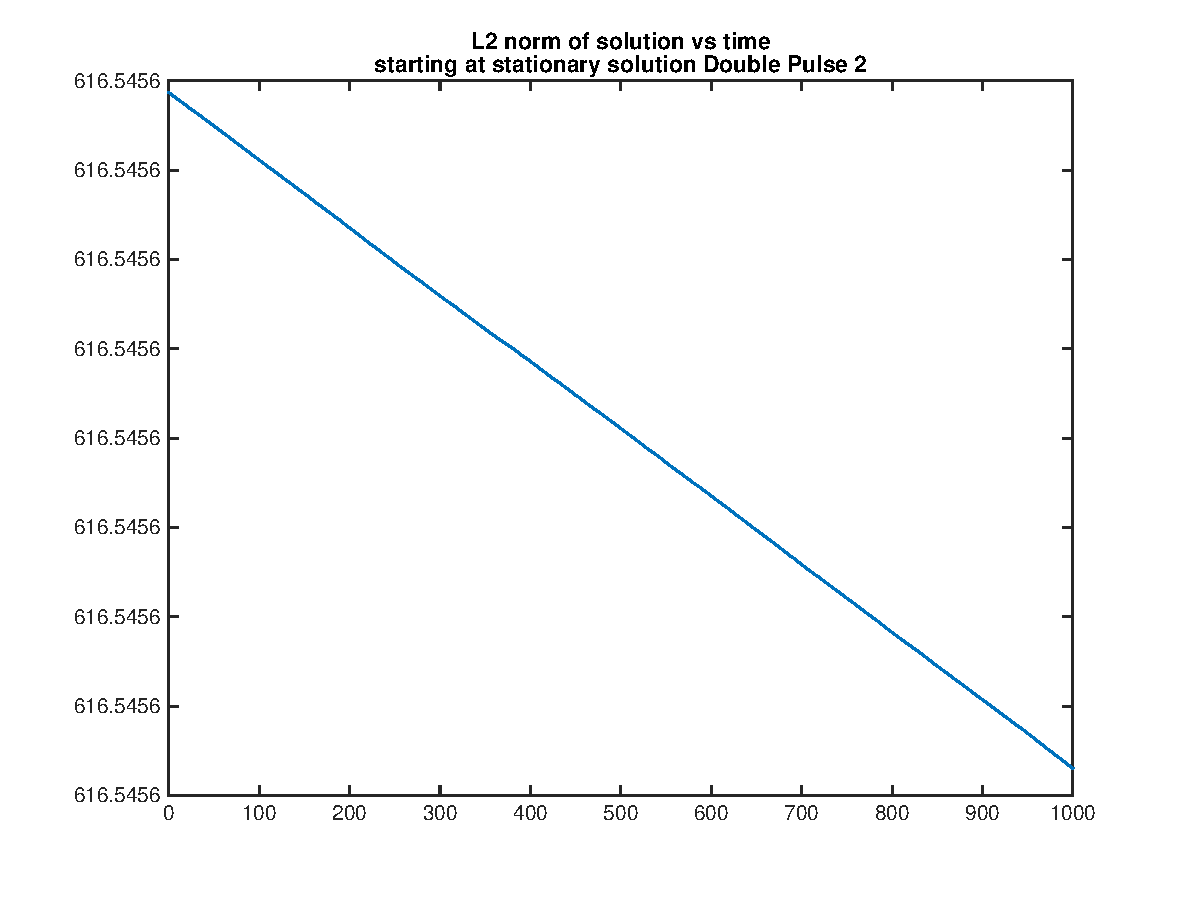
\includegraphics[width=8.5cm]{L2stationary1a.eps}
	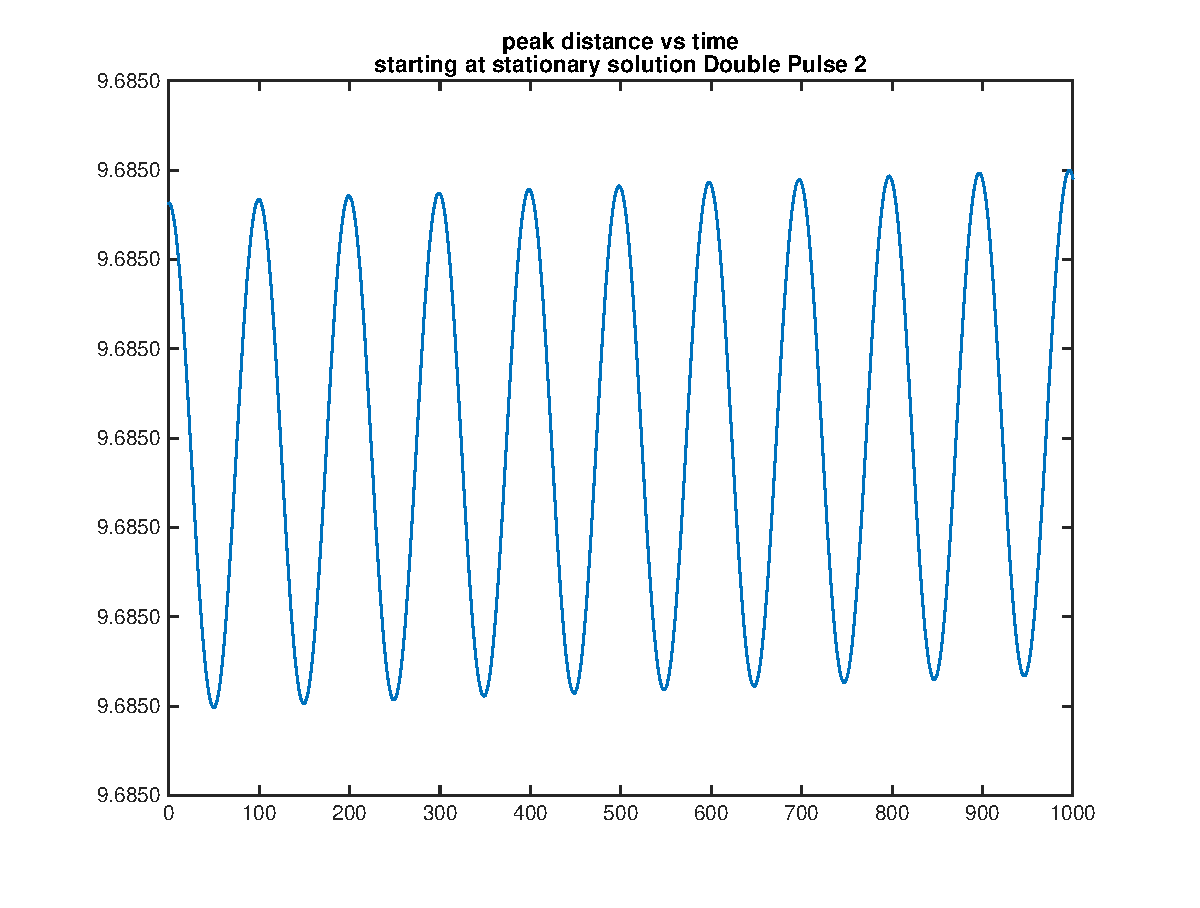
\includegraphics[width=8.5cm]{diststationary1a.eps}
\end{figure}

\subsubsection*{Chebyshev spectral methods}

Here we repeat what we have done using Chebyshev spectral methods instead of Fourier spectral methods. The idea is that the high frequency oscillations we obtained earlier resulted from oscillatory modes due to the essential spectrum being on the imaginary axis. We suspect that if we used nonperiodic BCs, we could eliminate these.\\

Since we are on a bounded interval $[-L, L]$, we choose Chebyshev spectral methods for our spatial discretization. Continuation code (to increase $c$) and double pulse construction are done using the 4th degree (integrated) KdV equation. The four boundary conditions are homogeneous Dirichlet and Neumann at both ends ($u(-L) = u(L) = u'(-L) = u'(L) = 0$). These are enforced by requring the polynomial interpolant be of the form $p(x) = (L^2 - x^2)q(x)$, where $q(x)$ satisfies the Dirichlet BCs at $\pm L$.\\

After running continuation code to $c = 9.4980$ (very close to a value we have used before), we construct our double pulses like we have in the past. For the 4th order equation, eigenvalue plots look as expected. For the 5th order equation, using Matlab's \texttt{eig}, we have the following eigenvalue plots. This plot is for Double Pulse 1, the first unstable double pulse. 

\begin{figure}[H]
	\includegraphics[width=8.5cm]{DP1eig.pdf}
	\includegraphics[width=8.5cm]{DP1eigzoom.pdf}
\end{figure}

Note that since we are using nonperiodic BCs, we have an absolute spectrum, which, when zoomed in, is not on the imaginary axis. (That is what we want.) It actually looks like the spectrum of the periodic version in an exponentially weighted space. We will return to this later and see if we can predict where this absolute spectrum lies. Since we know (roughly) the size of the eigenvalues (they are near 0), zooming in near 0 we find our eigenvalues.

\begin{figure}[H]
	\includegraphics[width=8.5cm]{DP1eignearorigin.pdf}
\end{figure}
Near 0, we have a double eigenvalue at the origin (eigenfunction is derivative of double pulse, as expected) and two small eigenvalues on either size of 0 which are negatives of each other. Their eigenfunctions look as expected from the periodic case (not shown).\\

Let's look at the eigenvalues we get for $c = 9.4980$. We use $N = 257$ grid points for our spatial discretization.

\begin{figure}[H]
\begin{tabular}{l|l}
Double Pulse   & Eigenvalues      \\ \hline
  1  &  $\pm 0.400$               \\ 
  2  &  2.9738e-08 $\pm 0.0631i$  \\ 
  3  & $\pm 0.0099$               \\
  4  & 6.5294e-12 $\pm 0.0030i$   \\
\end{tabular}
\end{figure}

As in the Fourier case, the real part for the complex eigenvalues is very small. Also as in the case, we can get rid of it using fsolve. In the table below, we see that there is a significant improvement in $\max (J -\lambda )f $ after using fsolve to eliminate the small real part of the eigenvalue. 

\begin{figure}[H]
\begin{tabular}{l|ll}
  Double Pulse  &  $\max (J -\lambda )f$ before \texttt{fsolve}  &  $\max (J -\lambda) f$ after \texttt{fsolve} \\ \hline
  2   &     1.1859e-06 &   7.2406e-09   \\ 
  4   &     2.2923e-06 &   2.8860e-10   \\ 
\end{tabular}
\end{figure}

\subsubsection*{Time Stepping}

Now we use our time-stepping method for the Chebyshev case. As before, we use the Crank-Nicolson/Adams Bashforth 2 IMEX scheme. Time step size is 0.01. For all plots we sample every 50 time steps, which is sufficient to produce good plots. No smoothing of any sort is needed, which is good, and a definite advantage of this method. \\

First we look at the solution starting exactly at Double Pulse 2. Here is a plot of the pulse distance as well as the derivative of the pulse distance vs pulse distance. Note the nice oscillations and nice orbit. We expect this to be a stationary solution, but it not quite one, likely due to numerical error. But since the orbit is really, really small, it is effectively a stationary solution.

\begin{figure}[H]
	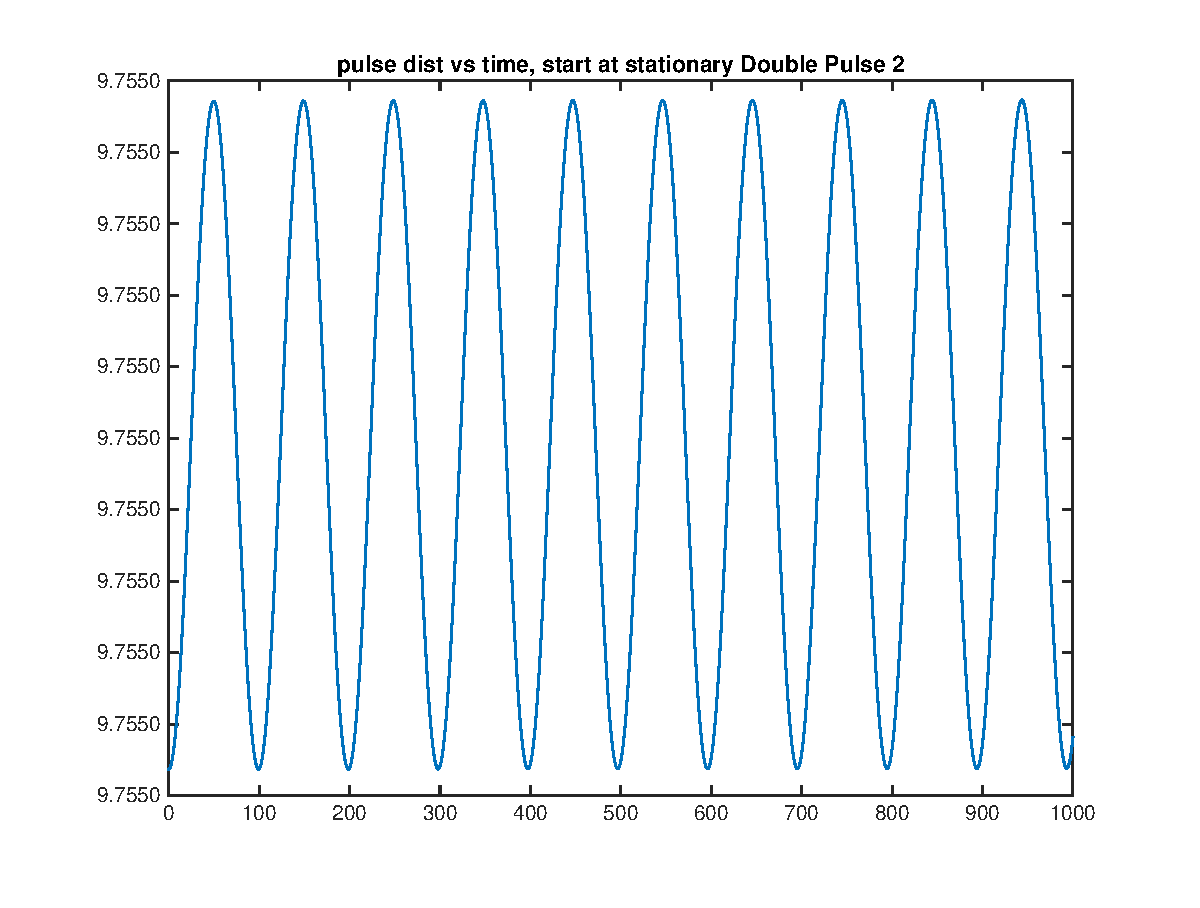
\includegraphics[width=8.5cm]{stat1a_dist}
	\includegraphics[width=8.5cm]{stat1a_orbit}
\end{figure}

We can also plot the energy (L2 norm) versus time. Note that the energy decays slightly with time, rather than being conserved, as we know it is. This is likely due to the numerical scheme.

\begin{figure}[H]
	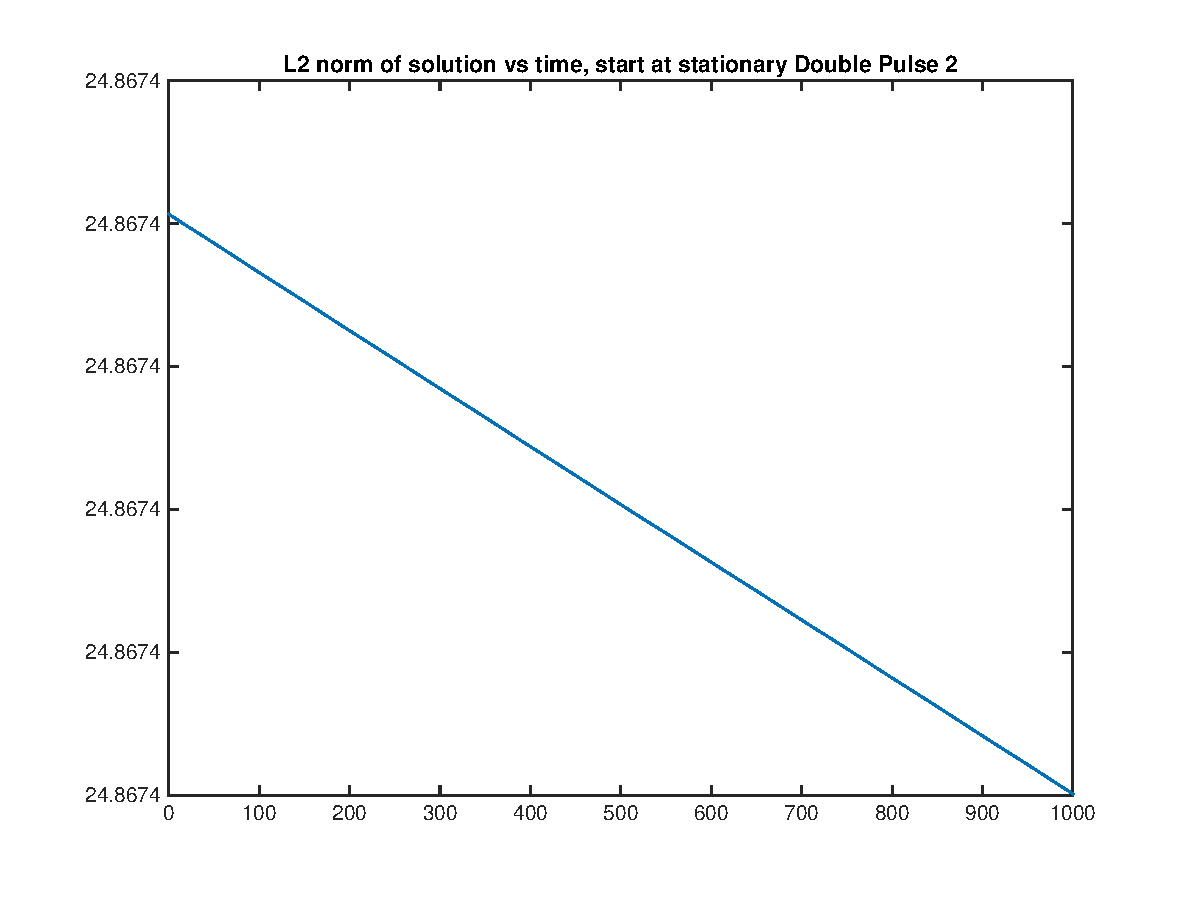
\includegraphics[width=8.5cm]{stat1a_norm}
\end{figure}

Now let's look at a solution near the stationary Double Pulse 2 solution. Again, we plot peak distance vs. time and derivative of peak distance vs peak distance.
\begin{figure}[H]
	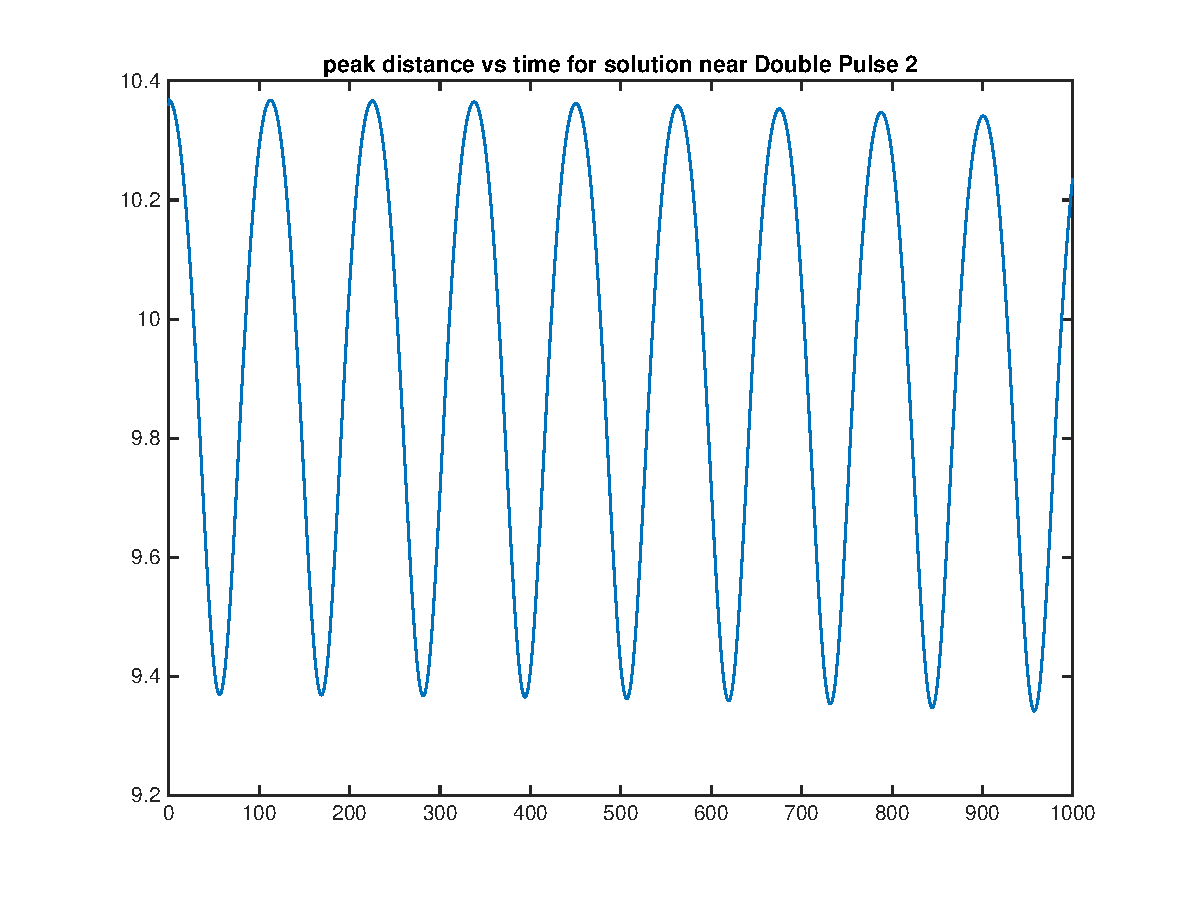
\includegraphics[width=8.5cm]{1a2dist}
	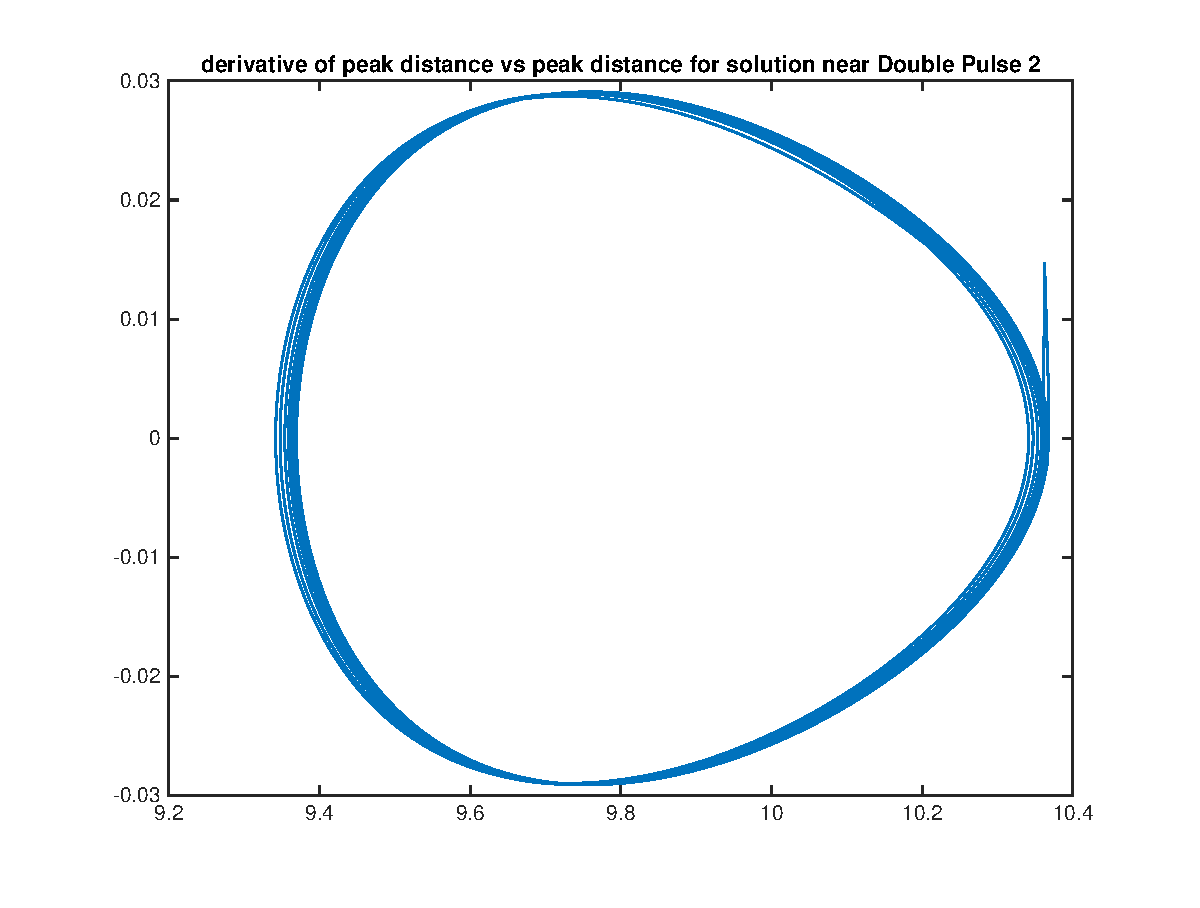
\includegraphics[width=8.5cm]{1a2deriv}
\end{figure}

It looks like a nice orbit, but it slowly moving to the left, i.e. decreasing in energy while the oscillation amplitudes remain the same. On the peak distance vs time plot, we can see the peak heights gradually decreasing. A plot of the energy shows a similar decrease. We start this plot after the norm has reached a stable pattern. We also cannot run it all the way, because our solution slowly translates to the left, and eventually runs into the boundary, where it disappears.

\begin{figure}[H]
	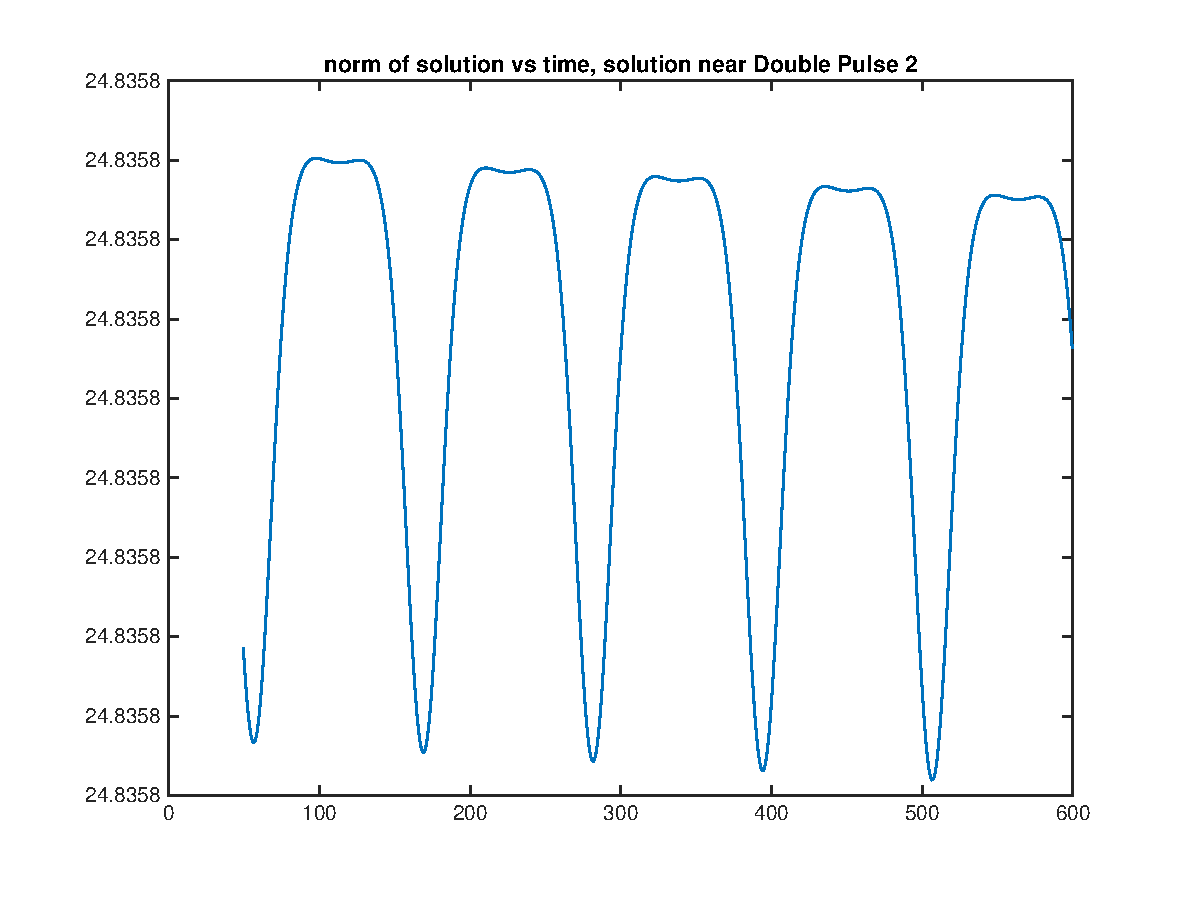
\includegraphics[width=8.5cm]{1a2norm}
\end{figure}

Here is another example. This time the pulses start farther apart than in the previous one. We plot derivative of peak distance vs peak distance.

\begin{figure}[H]
	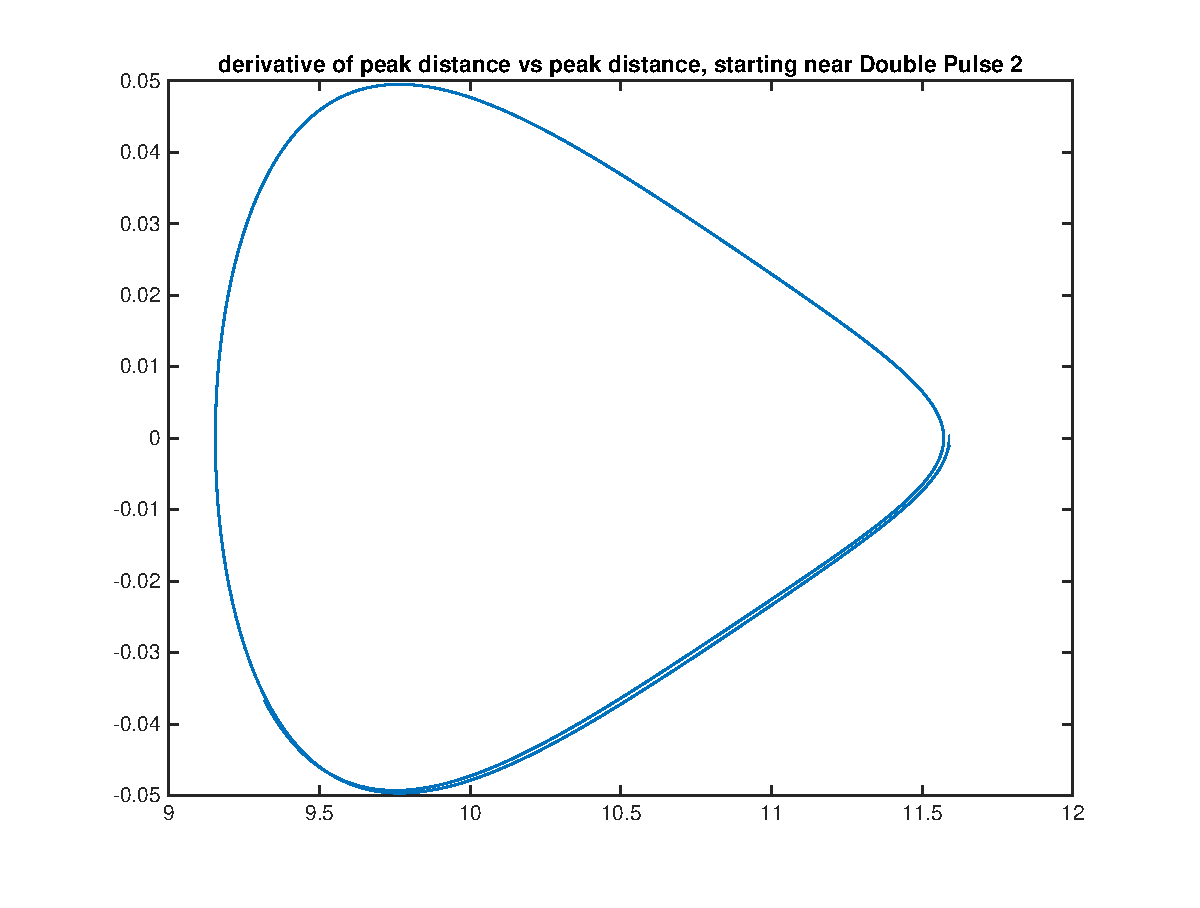
\includegraphics[width=8.5cm]{1a6deriv}
\end{figure}

We can see a nice orbit which again is moving slightly to the left as energy decreases, again likely from the numerical method.\\

At this point, we could construct a phase portrait similar to the Fourier case, but we would need to modify our code to keep the waves from running off the L boundary.



\end{document}